\section{Probability}
\label{sec:probability}

Probability theory and statistics can be traced back to as early as the 18th century. In 1718,~\citeauthor{ref:demoivre:1718}~\cite{ref:demoivre:1718} published the \textit{Doctrine of Chance}; a book that is widely regarded as the first published book on probability theory. In 1763, Thomas Bayes~\cite{ref:bayes:1763} published an article titled \textit{An Essay towards solving a Problem in the Doctrine of Chances} where the first version of \index{Bayes' theorem}Bayes' theorem was introduced.

Probability theory, statistics and \acf{ML} are transdisciplinary fields with many shared concepts. There are many examples of how probability theory has been incorporated into \acs{ML} research. In 1991,~\citeauthor{ref:denker:1991}~\cite{ref:denker:1991} proposed a way to transform \acf{ANN} outputs to probability distributions. In 1993, \citeauthor{ref:neal:1993}~\cite{ref:neal:1993} developed a \acf{MCMC} sampling algorithm for \acfp{BNN}. These are but a few examples of the role that probability theory has played in \acs{ML} research in the past.

Chapter \ref{chap:hhs} provided the concept of a \acf{HH}. This dissertation aims to develop a selection \acs{HH} that makes use of probability theory to select the best \acs{HH} to solve a given problem. This chapter aims to provide the necessary background information on probability theory and statistics. These are large fields and focus is put on the elements that are required to formulate the proposed \acf{BHH}.


\section{Overview of Probability}\label{sec:probability:overview}

In everyday conversation, the term \textit{probability} is a measure of belief in the occurrence of a future event~\cite{ref:wackerly:2014}. Probability is a necessary tool used in many fields including physics, biology, chemistry and computer science. These fields contain many cases that generate observations that cannot be predicted with absolute certainty~\cite{ref:wackerly:2014}. Probability can be inferred and confirmed through past events. These events are referred to as \textit{random} or \textit{stochastic} events. The probability that a certain event, $A$, might occur is denoted by $P(A)$. Although these random events cannot be predicted with absolute certainty, the relative frequency with which they occur over many trials, is often remarkably stable.

Consider flipping an unbiased, fair coin. The coin has two possible outcomes. It can conclude that each side has a $\frac{1}{2}$ or $50\%$ chance of occurring. In statistics, the decimal probability notation is used, where $0 <= P(A) <= 1$. Suppose the fair coin is thrown 10 times, there is no guarantee of observing $0.5$ heads and $0.5$ tails. There is some probability (although small) that the coin might fall on heads $0/10$ times. The probability of such an event occurring is $0.0009765625$. In the coin flip example, the \acf{CLT} shows that the normalised sum of events tends toward a normal distribution with a mean value of $0.5$, if the number of events observed, $N$, is large~\cite{ref:wackerly:2014}. The larger the value of $N$, the higher the confidence of mean probability and relative frequency of the event. The stable long-term relative frequency by which a random event occurs, provides an intuitive and meaningful measure of belief that a certain event will occur again at some point in the future~\cite{ref:wackerly:2014}.

Probability can also be expressed over multiple random events. Multiple random events can be considered together, dependently or conditionally. The following sections provide insight into conditional and joint probabilities of multiple random events.

\index{Bayes' theorem}
\begin{theorem}[\textbf{Bayes' theorem}]
	\label{th:probability:bayes_theorem:theorem}
	Assume that $\{B_{1}, B_{2}, \dots, B_{K}\}$ is a partition of $S$ such that $P(B_{i}) > 0$, for $i = 1,2, \dots, K$ then\\
	\\
	\begin{equation}
		P(B_{j} \vert A) = \frac{P(A \vert B_{j})P(B_{j})}{\sum_{i=1}^{K} P(A \vert B_{i})P(B_{i})}
	\end{equation}
\end{theorem}

\begin{proof}
	The proof follows from the definition of conditional probability as was presented in Section~\ref{sec:probability:cond_probability}:

	\begin{equation}
		\begin{split}
			P(B_{j} \vert A)
			&= \frac{P(A \cap B_{j})}{P(A)}\\
			&= \frac{P(A \vert B_{j})P(B_{j})}{\sum_{i=1}^{K} P(A \vert B_{i})P(B_{i})}
		\end{split}
	\end{equation}
\end{proof}

One of the many applications of \index{Bayes' theorem}Bayes' theorem is to do statistical inference. \index{Bayes' theorem}Bayes' theorem expresses how a degree of belief, expressed as a probability, should rationally change to account for the availability of related evidence.



\section{Conjugate Priors}\label{sec:probability:conjugate_priors}

\citeauthor{ref:wackerly:2014}\cite{ref:wackerly:2014} state that conjugate priors are prior probability distributions that result in posterior distributions that are of the same functional form, $\mathcal{A}(v)$, as the prior, but with different parameter values. This section considers the conjugate priors that are used with the Binomial likelihood and Categorical/Multinomial likelihood.

\subsection{Binomial Likelihood}\label{sec:probability:conjugate_priors:binom_likelihood}

The conjugate prior to a \index{Bernoulli probability distribution}Bernoulli probability distribution is the \index{Beta probability distribution}Beta probability distribution
\cite{ref:wackerly:2014}. This is shown by demonstrating that the posterior distribution has the
same functional form, $\mathcal{A}(v)$, as the prior distribution as follows. \\\\
\textbf{Setup}:

\begin{itemize}
	\item Let $I$ be a number of independent, identical  (iid) random events.

	\item Let $\alpha \in \mathbb{R}, \alpha > 0$ and $\beta \in \mathbb{R}, \beta >0$ be the shape parameters to the \index{Beta probability distribution}Beta probability distribution.

	\item Let $\theta$ be the probability of a success. With $\theta | \alpha, \beta \sim Beta(\alpha, \beta)$.

	\item $P(\theta)$ is the prior probability distribution with the functional form $\mathcal{A}(v)$.

	\item Let $\boldsymbol{X} = (x_{1}, \dots, x_{I})$ be the outcomes of $I$ independent, identical random events, each with Boolean outcome. That is $x_{i} | \theta \overset{\text{iid}}{\sim} Ber(\theta)$ and $\mathcal{L}(x_{i} \vert \theta)$ is the Bernoulli likelihood.

	\item Let $\boldsymbol{\mathcal{D}}$ denote all the prior data of $\boldsymbol{X}$, parameterised by $\alpha$, $\beta$.

	\item Let $N_{1} = \sum_{i=1}^{I} \mathbbm{1}(x_{i} = 1)$ and $N_{0} = \sum_{i=1}^{I} \mathbbm{1}(x_{i} = 0)$.
\end{itemize}

The Bernoulli likelihood is given as

\begin{equation}
	\label{eq:probability:conjugate_priors:binom_likelihood:likelihood}
	\begin{split}
		\mathcal{L}(\boldsymbol{\mathcal{D}}) &=  P(\boldsymbol{\mathcal{D}} | \theta) \\
		&\propto \theta^{N_{1}}(1-\theta)^{N_{0}}
	\end{split}
\end{equation}

By \index{Bayes' theorem}Bayes' theorem, the posterior distribution with given prior data $\boldsymbol{\mathcal{D}}$ is given as

\begin{equation}
	\begin{split}
		\label{eq:probability:conjugate_priors:binom_likelihood:posterior}
		P(\theta \vert \boldsymbol{\mathcal{D}}) &= \frac{P(\boldsymbol{\mathcal{D}} | \theta) P(\theta)}{P(\boldsymbol{\mathcal{D}})}
	\end{split}
\end{equation}

Since the denominator sums to $1$, the denominator and constants for the Bernoulli likelihood and the Beta prior can be removed by expressing the posterior as proportional to the likelihood times the prior as follows:

\begin{equation}
	\label{eq:probability:conjugate_priors:binom_likelihood:posterior_propto}
	\begin{split}
		P(\theta | \boldsymbol{\mathcal{D}}) &\propto \left[\theta^{N_{1}}(1-\theta)^{N_{0}}\right] \left[\theta^{\alpha - 1} (1 - \theta)^{\beta - 1}\right] \\
		&\propto \theta^{(N_{1} + \alpha) - 1}(1-\theta)^{(N_{0} + \beta) - 1} \\
		&\propto Beta(N_{1} + \alpha, N_{0} + \beta)
	\end{split}
\end{equation}

The posterior distribution has the same functional form, $\mathcal{A}(v)$, as the prior, but with updated prior parameters $\alpha' = N_{1} + \alpha$ and $\beta' = N_{0} + \beta$. This shows that the \index{Beta probability distribution}Beta probability distribution is the conjugate prior used with the Bernoulli likelihood.


\subsection{Categorical and Multinomial Likelihood}
\label{sec:probability:conjugate_priors:cat_mult_likelihood}

The conjugate prior to a \index{Categorical probability distribution}Categorical and \index{Multinomial probability distribution}Multinomial probability distribution is the \index{Dirichlet probability distribution}Dirichlet probability distribution~\cite{ref:wackerly:2014}. The proof of the conjugate prior for the \index{Bernoulli probability distribution}Bernoulli probability distribution is similar to the proof presented in Section \ref{sec:probability:conjugate_priors:binom_likelihood}. This means that the posterior distribution must have the same functional form, $\mathcal{A}(v)$, as the prior distribution. The proof is shown as follows. \\\\
\textbf{Setup}:

\begin{itemize}
	\item Let $I$ be a number of independent, identical (iid) random events.

	\item Let $K$ be a number of possible outcomes for each event, with $K \geq 2$.

	\item Let $\boldsymbol{\alpha} = (\alpha_{1}, \dots, \alpha_{K}), \forall_{k=1}^{K} \alpha_{k} \in \mathbb{R}, \alpha_{k} > 0$ be the concentration parameters to the \index{Dirichlet probability distribution}Dirichlet probability distribution.

	\item Let $\boldsymbol{\theta} = (\theta_{1}, \dots, \theta_{K}), \forall_{k=1}^{K} \theta_{k} \in (0,1), \sum_{k}^{K} \theta_{k} = 1$ be the probability of each class in $K$ and $\boldsymbol{\theta}$ belongs to the standard $K-1$ probability simplex $S$. With $\boldsymbol{\theta} | \boldsymbol{\alpha} \sim Dir(K, \boldsymbol{\alpha})$.

	\item $P(\boldsymbol{\theta})$ is the prior probability distribution with the functional form $\mathcal{A}(v)$.

	\item Let $\boldsymbol{X} = (\boldsymbol{x_{1}}, \dots, \boldsymbol{x_{I}})$ be the outcomes of $I$ independent, identical random events, each with $K$ possible outcomes. That is $\boldsymbol{x_{i}} | \boldsymbol{\theta} \overset{\text{iid}}{\sim} Cat(\boldsymbol{\theta})$ and $\mathcal{L}(\boldsymbol{x_{i}} \vert \boldsymbol{\theta})$ is the Categorical likelihood.

	\item Let $\boldsymbol{\mathcal{D}}$ denote all the prior data of $\boldsymbol{X}$, parameterised by $\boldsymbol{\alpha}$.

	\item Let $\boldsymbol{N} = (N_{1}, \dots, N_{K}), N_{k} = \sum_{i=1}^{I} \mathbbm{1}(x_{i,k} = 1)$, denote the counts for each occurrence of a class $k$.
\end{itemize}

The likelihood of the Categorical and \index{Multinomial probability distribution}Multinomial probability distributions is given as

\begin{equation}
	\label{eq:probability:conjugate_priors:mult_likelihood:likelihood}
	\begin{split}
		\mathcal{L}(\boldsymbol{\mathcal{D}}) &=  P(\boldsymbol{\mathcal{D}} | \boldsymbol{\theta}) \\
		&\propto \prod_{k=1}^{K} \theta_{k}^{N_{k}}
	\end{split}
\end{equation}

By \index{Bayes' theorem}Bayes' theorem, the posterior distribution with given prior data $\boldsymbol{\mathcal{D}}$ is given as

\begin{equation}
	\label{eq:probability:conjugate_priors:mult_likelihood:posterior}
	\begin{split}
		P(\boldsymbol{\theta} \vert \boldsymbol{\mathcal{D}}) &= \frac{P(\boldsymbol{\mathcal{D}} \vert \boldsymbol{\theta}) P(\boldsymbol{\theta)}}{P(\boldsymbol{\mathcal{D}})}
	\end{split}
\end{equation}

Since the denominator sums to $1$, the denominator and constants for the \index{Dirichlet probability distribution}Dirichlet prior can be removed by expressing the posterior as proportional to the likelihood times the prior as follows:

\begin{equation}
	\label{eq:probability:conjugate_priors:mult_likelihood:posterior_propto}
	\begin{split}
		P(\boldsymbol{\theta} \vert \boldsymbol{\mathcal{D}}) &\propto \prod_{k=1}^{K} \theta_{k}^{N_{k}} \prod_{k=1}^{K} \theta_{k}^{\alpha_{k} - 1}\\
		&\propto \prod_{k=1}^{K} \theta_{k}^{(N_{k} + \alpha_{k}) - 1} \\
		&\propto Dir(K, \boldsymbol{N} + \boldsymbol{\alpha})
	\end{split}
\end{equation}

The posterior distribution has the same form, $\mathcal{A}(v)$, as the prior, but with updated prior parameters $\boldsymbol{\alpha'} = \boldsymbol{N} + \boldsymbol{\alpha}$. This shows that the \index{Dirichlet probability distribution}Dirichlet probability distribution is the conjugate prior used with the Categorical/Multinomial likelihood.

\section{Bayesian Statistics}
\label{sec:probability:bayesian_statistics}

This section provides detailed discussions on various aspects related to Bayesian statistics and probability. Brief discussion follow on the frequentist and the Bayesian approach to statistics and probability. Finally, the concept of Bayesian analysis is presented in detail.

\subsection{Frequentist vs. Bayesian Statistics}
\label{sec:probability:bayesian_statistics:frequentist_vs_bayesian}

In general, there are two main views to probability and statistics. These include the \textit{frequentist} and the \textit{Bayesian} view of statistics. Naturally, Bayesian statistics is based on \index{Bayes' theorem}Bayes' theorem as was presented in Section \ref{sec:probability:bayes_theorem}. Bayesian statistics describe the probability of an event in terms of some belief, based on previous knowledge of the event and the conditions under which the event happened~\cite{ref:hackenberger:2019}. To introduce the concept of Bayesian inference and Bayesian analysis, the differences between the frequentist and the Bayesian view of statistics need to be presented.

Bayesian statistics out-date the frequentist approach, but lacked interest in the early days, partly because of the limited applications where the conjugate priors where known~\cite{ref:hackenberger:2019}. More recent advancements in mathematical methods popularised the Bayesian approach again. A notable contribution to this switch was the development of the \acf{MCMC} algorithm in the 1950s. This family of algorithms allowed for the construction of random sampling algorithms from a probability distribution, which allows for the calculation of Bayesian hierarchical models~\cite{ref:hackenberger:2019}. Soon after followed one of the earliest papers that use Bayesian statistics in the field of medicine in 1982~\cite{ref:ashby:2006}.

The difference between the frequentist approach and the Bayesian approach can be illustrated using an example.~\citeauthor{ref:hackenberger:2019}~\cite{ref:hackenberger:2019} suggests an experiment that investigates whether the gender ratio in some hypothetical mice population is $1:1$. Two experiments were designed. In the first experiment, mice are randomly selected until the first male is chosen. The result in this experiment will then be the total number of mice chosen by gender. For the second experiment, exactly seven mice are randomly selected. The result of the second experiment would be the number of males and females in a sample of seven. Suppose the outcome of the experiment was $FFFFFFM$, where $F$ represents a female and $M$ represents a male. If the experimental design is not known ahead of time, the result is useless. Consider the $p$-value for each of these experiments. The $p$-value is the probability of obtaining results at least as extreme as the observed results of a statistical hypothesis test~\cite{ref:thisted:1998}. For the first experiment, the $p$-value is $0.031$ and for the second experiment, the $p$-value is $0.227$. Using a confidence level of $\alpha = 0.05$, opposite outcomes could be concluded for these two experiments when it comes to rejecting the null hypothesis, despite using the same data. The reason for the difference in outcomes, is due to the difference in their null distributions, which represent the probability distribution of the test statistic when the null hypothesis is true. The first approach uses a geometrical approach, and the second used a binomial approach as illustrated in Figure \ref{fig:probability:bayesian_statistics:mouse_experiment_outcome}.

\begin{figure}[htb]
	\centering
	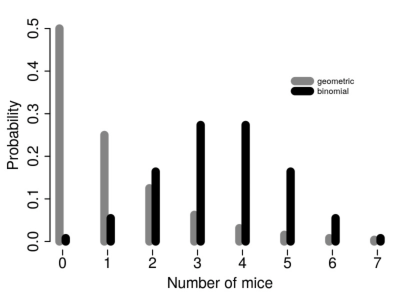
\includegraphics[width=0.6\textwidth]{images/mouse_experiment_outcome.pdf}
	\caption{The experimental outcomes for the mice-population experiments as was taken from~\cite{ref:hackenberger:2019} .}
	\label{fig:probability:bayesian_statistics:mouse_experiment_outcome}
\end{figure}

If Bayesian statistics is used, the experimental design that was chosen does not matter. In Bayesian statistics it is common to use a \index{Beta probability distribution}Beta probability distribution as a prior distribution. If the prior distribution is sampled from $Beta(3,3)$, then using Bayesian analysis, the posterior distribution, according to the outcomes of this experiment, would yield $Beta(9,4)$.

~\citeauthor{ref:hackenberger:2019}~\cite{ref:hackenberger:2019} mentions that the $Beta$ probability distribution can be seen as a probability distribution of the occurrence of specific parameters. From the information that is now known about the $Beta$ probability distribution, it is possible to calculate the probability that the gender ratio in this mice population is not $1:1$, with the $Beta$ probability distribution as a prior, yielding a $p$-value of $0.92$. This means that there is a probability of $92\%$ that the mice population is not $1:1$, regardless of experimental design. An illustration of this is given in Figure \ref{fig:probability:bayesian_statistics:mouse_distributions}.

\begin{figure}[htbp]
	\centering
	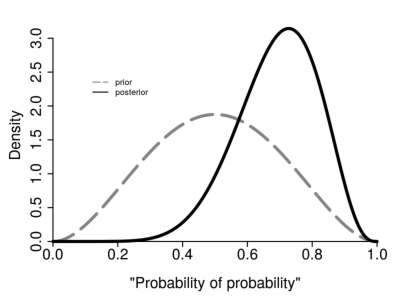
\includegraphics[width=0.6\textwidth]{images/mouse_experiment_distributions.pdf}
	\caption{An illustration of the prior and posterior probability distributions for the outcomes of the mice-population experiment, using a $Beta$ prior, as was taken from~\cite{ref:hackenberger:2019}.}
	\label{fig:probability:bayesian_statistics:mouse_distributions}
\end{figure}

Figure \ref{fig:probability:bayesian_statistics:mouse_distributions} shows how the posterior distribution differs from the prior distribution.

\subsection{Bayesian Analysis}
\label{sec:probability:bayesian_statistics:bayesian_analysis}

Bayesian analysis is the process by which prior beliefs are updated as a result of observing new data/evidence. Similar to the approaches followed above to explain Bayesian statistics, a proposal is made to explain Bayesian analysis by means of an example taken from~\cite{ref:wackerly:2014}. Let $\boldsymbol{Y} = (Y_{1}, Y_{2}, \dots, Y_{N})$ denote the random variable that is observed over a sample size of $N$. Then the likelihood of the sample is given as $\mathcal{L}(y_{1}, y_{2}, \dots, y_{n} \vert \theta)$. In the discrete case, the likelihood function is defined to be the joint probability, $P(Y_{1} = y_{1}, Y_{2} = y_{2}, \dots, Y_{N} = y_{n})$, and for the continuous case, yields the joint density of $Y_{1}, Y_{2}, \dots, Y_{N}$, evaluated at $y_{1}, y_{2}, \dots, y_{n}$. The Bayesian view models the parameter $\theta$ as a random variable with a probability distribution, referred to as the prior distribution of $\theta$. The symbol $\theta$, is included in the notation of $\mathcal{L}$ as an argument to illustrate that this function is dependent, explicitly, on the value of $\theta$. Importantly, the prior distribution is specified before any data is collected and represents the theoretical prior knowledge about $\theta$. Assume that the parameter $\theta$ has a continuous distribution with density $g(\theta)$ that has no unknown parameters. Considering the likelihood of the data and the prior on $\theta$, then the joint likelihood of $Y_{1}, Y_{2}, \dots, Y_{N}, \theta$ is given as

\begin{equation}
	\label{eq:probability:bayesian_statistic:bayesian_analysis:joint_likelihood}
	f(y_{1}, y_{2}, \dots, y_{n}, \theta) = \mathcal{L}(y_{1}, y_{2}, \dots, y_{n} \vert \theta)g(\theta)
\end{equation}

The marginal density or mass function of $Y_{1}, Y_{2}, \dots, Y_{N}$ is given as

\begin{equation}
	\label{eq:probability:bayesian_statistic:bayesian_analysis:marginal_density}
	m(y_{1}, y_{2}, \dots, y_{n}) = \int_{-\infty}^{\infty} \mathcal{L}(y_{1}, y_{2}, \dots, y_{n} \vert \theta)g(\theta)d\theta
\end{equation}

Finally, the posterior density of $\theta \vert y_{1}, y_{2}, \dots, y_{n}$ denoted by $g^{*}(\theta \vert y_{1}, y_{2}, \dots, y_{n})$, according to \index{Bayes' theorem}Bayes' theorem, is given as

\begin{equation}
	\label{eq:probability:bayesian_statistic:bayesian_analysis:posterior_density}
	g^{*}(\theta \vert y_{1}, y_{2}, \dots, y_{n}) = \frac{\mathcal{L}(y_{1}, y_{2}, \dots, y_{n} \vert \theta)g(\theta)}{\int_{-\infty}^{\infty} \mathcal{L}(y_{1}, y_{2}, \dots, y_{n} \vert \theta)g(\theta)d\theta}
\end{equation}

\citeauthor{ref:wackerly:2014}\cite{ref:wackerly:2014} mention that the posterior density summarises all the pertinent information about the parameter $\theta$ by making use of the information contained in the prior for $\theta$, as well as the information in the observed data/evidence.

Consider now how Bayesian analysis can be used to update the priors on $\theta$ based on newly observed data. As with the example above, the discussion below is taken from~\cite{ref:wackerly:2014}. Let $Y_{1}, Y_{2}, \dots, Y_{N}$ denote a random sample from a \index{Bernoulli probability distribution}Bernoulli probability distribution, where $P(Y_{i} = 1) = \theta$ and $P(Y_{i} = 0) = 1 - \theta$ and the prior distribution for $\theta$ is $Beta(\alpha, \beta)$. The posterior distribution for $\theta$ can be formulated as follows. The Bernoulli probability function is written as

\begin{equation}
	\label{eq:probability:bayesian_statistic:bayesian_analysis:step_1}
	P(y_{i} \vert \theta) = \theta^{y_{i}}(1 - \theta)^{1-y_{i}}
\end{equation}

where $y_{i} = \{0,1\}$ and $0 < \theta < 1$. The likelihood $\mathcal{L}(y_{1}, y_{2}, \dots, y_{n} \vert \theta)$ is presented as follows:

\begin{equation}
	\label{eq:probability:bayesian_statistic:bayesian_analysis:step_2}
	\begin{split}
		\mathcal{L}(y_{1}, y_{2}, \dots, y_{n} \vert \theta)
		&= P(y_{1}, y_{2}, \dots, y_{n} \vert \theta)\\
		&= \theta^{y_{1}}(1-\theta)^{1 - y_{1}} \times \theta^{y_{2}}(1-\theta)^{1 - y_{2}} \times \dots \times \theta^{y_{n}}(1-\theta)^{1 - y_{n}}\\
		&= \theta^{\sum y_{i}}(1-\theta)^{n-\sum y_{i}}
	\end{split}
\end{equation}

Then the joint likelihood of $Y_{1}, Y_{2}, \dots, Y_{N}, \theta$ from Equation~\eqref{eq:probability:bayesian_statistic:bayesian_analysis:joint_likelihood} is formulated as

\begin{equation}
	\label{eq:probability:bayesian_statistic:bayesian_analysis:step_3}
	\begin{split}
		f(y_{1}, y_{2}, \dots, y_{n}, \theta)
		&= \mathcal{L}(y_{1}, y_{2}, \dots, y_{n} \vert \theta)g(\theta)\\
		&= \theta^{\sum y_{i}}(1-\theta)^{n-\sum y_{i}} \times \frac{\Gamma(\alpha + \beta)}{\Gamma(\alpha)\Gamma(\beta)}\theta^{\alpha - 1}(1 - \theta)^{\beta  - 1}\\
		&= \frac{\Gamma(\alpha + \beta)}{\Gamma(\alpha)\Gamma(\beta)}\theta^{\sum y_{i} + \alpha - 1}(1-\theta)^{n - \sum y_{i} + \beta - 1}
	\end{split}
\end{equation}

The marginal density of $Y_{1}, Y_{2}, \dots Y_{N}$ is then given as

\begin{equation}
	\label{eq:probability:bayesian_statistic:bayesian_analysis:step_4}
	\begin{split}
		m(y_{1}, y_{2}, \dots, y_{n})
		&= \int_{0}^{1}\frac{\Gamma(\alpha + \beta)}{\Gamma(\alpha)\Gamma(\beta)}\theta^{\sum y_{i} + \alpha - 1}(1-\theta)^{n - \sum y_{i} + \beta - 1}d\theta\\
		&= \frac{\Gamma(\alpha + \beta)}{\Gamma(\alpha)\Gamma(\beta)}\frac{\Gamma(\sum y_{i} + \alpha)\Gamma(n - \sum y_{i} + \beta)}{\Gamma(n + \alpha + \beta)}
	\end{split}
\end{equation}

Finally, the posterior density of $\theta$, denoted by $g^{*}(\theta \vert y_{1}, y_{2}, \dots, y_{n})$, is given as

\begin{equation}
	\label{eq:probability:bayesian_statistic:bayesian_analysis:step_5}
	\begin{split}
		g^{*}(\theta \vert y_{1}, y_{2}, \dots, y_{n})
		&= \frac{\frac{\Gamma(\alpha + \beta)}{\Gamma(\alpha)\Gamma(\beta)}\theta^{\sum y_{i} + \alpha - 1}(1-\theta)^{n - \sum y_{i} + \beta - 1}}{\frac{\Gamma(\alpha + \beta)}{\Gamma(\alpha)\Gamma(\beta)}\frac{\Gamma(\sum y_{i} + \alpha)\Gamma(n - \sum y_{i} + \beta)}{\Gamma(n + \alpha + \beta)}}\\
		&= \frac{\Gamma(n + \alpha + \beta)}{\Gamma(\sum y_{i} + \alpha)\Gamma(n - \sum y_{i} + \beta)}\theta^{\sum y_{i} + \alpha - 1}(1-\theta)^{n - \sum y_{i} + \beta - 1}
	\end{split}
\end{equation}

The posterior density has the same functional form, $\mathcal{A}(v)$, as the prior, yielding the update on prior parameters as $\alpha' = \sum y_{i} + \alpha$ and $\beta' = n - \sum y_{i} + \beta$.

